\chapter{Methodology}
In this Chapter, how the models are constructed will be elaborated, starting with the Data Collection in Section \ref{data_collection}. The data of site 15 will be split into two parts, 2001-2008 for the training, and 2009 and 2010 will be the testing years. The second Section \ref{mathematical models} shows the Mathematical equations for the three models. Together with the Flowcharts in Section\ref{flowcharts} they form the foundation on how the models are constructed. The actual Model Development will be elaborated on in Section \ref{model development}, first the data preprocessing, then the Hybrid ARIMA-ANN model, then the BNN with MCD model and finally the LSTM model. Finally, Section \ref{evaluation metrics method} explains how the models can be quantified and which Evaluation Metrics are used for this. 

\section{Data Collection}
\label{data_collection}
The data will be used for the model's training/learning and testing phases. One site, 15 North Sea Center, is used for measurements, with the help of buoys equipped with sensors. The site gathered information for 10 years, with a measurement of each hour of each day for a total of 87,600 data points. An example of one time step of the measurements can be seen in Table \ref{table:metocean_data}. The depth of the site is $29$ meters and is located in the middle of the North Sea, Figure \ref{fig:location buoys} shows the location of site 15. For seabed wind turbines, which are installed between $0-30$ meters, it would not be relevant to investigate deeper sites (\cite{DNV2018}).

\begin{figure}[ht!]
    \centering
    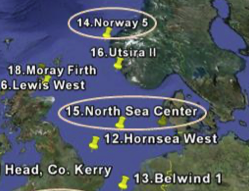
\includegraphics[width=0.4\linewidth]{images/Location buoys.png}
    \caption{Location buoys (\cite{lin2015joint})}
    \label{fig:location buoys}
\end{figure}

\begin{table}[ht!]
\centering
\caption{Met-ocean Data hour 1}
\renewcommand{\arraystretch}{1.5} % Adjust row spacing
\resizebox{\textwidth}{!}{%
\begin{tabular}{|c|c|c|c|c|c|c|c|c|}
\hline
\textbf{nx} & \textbf{ny} & \textbf{datetime} & \textbf{s\_wht} & \textbf{meanwdir} & \textbf{peak\_fr} & \textbf{mean\_fr} & \textbf{ustar} & \textbf{wind\_dir} \\
\hline
470 & 584 & 1/1/01 0:00 & 2.16 & 168.336 & 0.175 & 0.194 & 0.693 & 168.313 \\
\hline
\textbf{cdg} & \textbf{wind\_speed} & \textbf{depth} & \textbf{maxwh} & \textbf{maxwp} & \textbf{swe\_h} & \textbf{meansdir} & \textbf{meansfr} & \textbf{wsea\_h} \\
\hline
0 & 17.278 & 29 & 4.679 & 4.878 & 0.31 & 131.235 & 0.17 & 2.14 \\
\hline
\textbf{wsead} & \textbf{wsea\_fr} & \textbf{msp1} & \textbf{msp2} & \textbf{mwseap1} & \textbf{mwseap2} & & & \\
\hline
168.642 & 0.195 & 5.674 & 5.552 & 4.73 & 4.401 & & & \\
\hline
\end{tabular}%
}
\label{table:metocean_data}
\end{table}

\noindent From this data the significant wave height, $s_{wht}$, the wind speed, $wind_{speed}$, the mean frequency, $mean_{fr}$, and the datetime will be used. The reasoning follows from earlier research, Boer and Overvliet (\cite{boer2022installation}, \cite{overvliet2023uncertainty}), who already found the significance of these parameters in the installation phase of the turbines. While other parameters influence these key parameters, they fall beyond this project's scope. The installing ships can only be used when the values do not go over the operational limits of Table \ref{table:operational_limits}. The location of the site can be seen in Figure \ref{fig:location buoys}, site $15$ corresponds to a depth of $29$ meters. \\

\noindent To show the relevance of these models in respect to the jack-up vessels maximum values-on the significant wave heigth $=2.5$ [meters], the wind speed $=16$, $10$ and $8$ [meters per second] and the mean period for the crane barge or the heavy lift vehicle (HVL) $=9$ and $7$ [seconds]-these values over the mean of the available data is shown in Figure \ref{fig:site15_limits}. Some trends are already visible in these figures. Firstly, seasonality where hour $0$ represents the $1^{st}$ of January at 00:00. The peaks at the winter months are significantly higher than those in summer. Another recurring trend is the increasing difference between the minimum and maximum values of each peak over time. This is especially visible in the significant wave height and the mean frequency, which can probably be linked to the tides. 

\begin{figure}[h!]
    \centering
    \begin{subfigure}[b]{0.47\textwidth}
        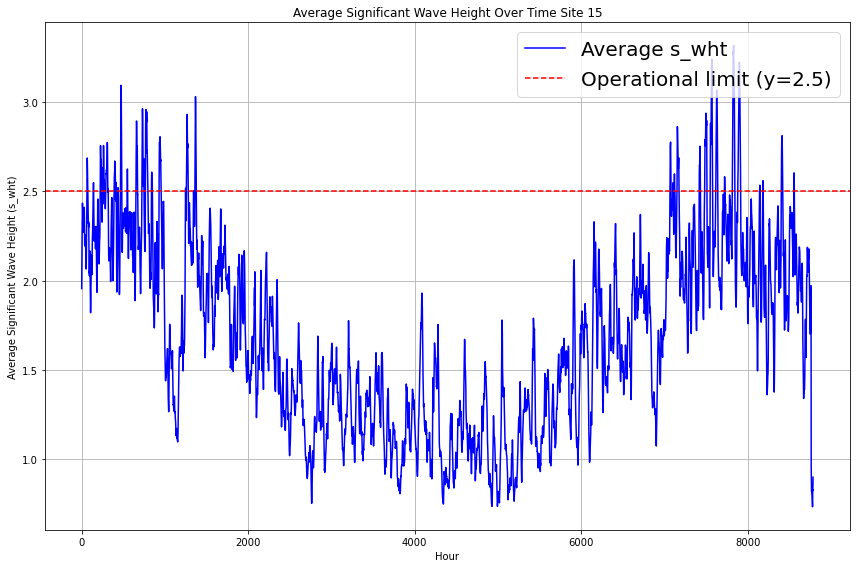
\includegraphics[width=\textwidth]{graphs/s_wht_limit_site_15.png} 
        \caption{Significant Wave Height}
        \label{fig:s_wht_15}
    \end{subfigure}
    \hfill
    \begin{subfigure}[b]{0.47\textwidth}
        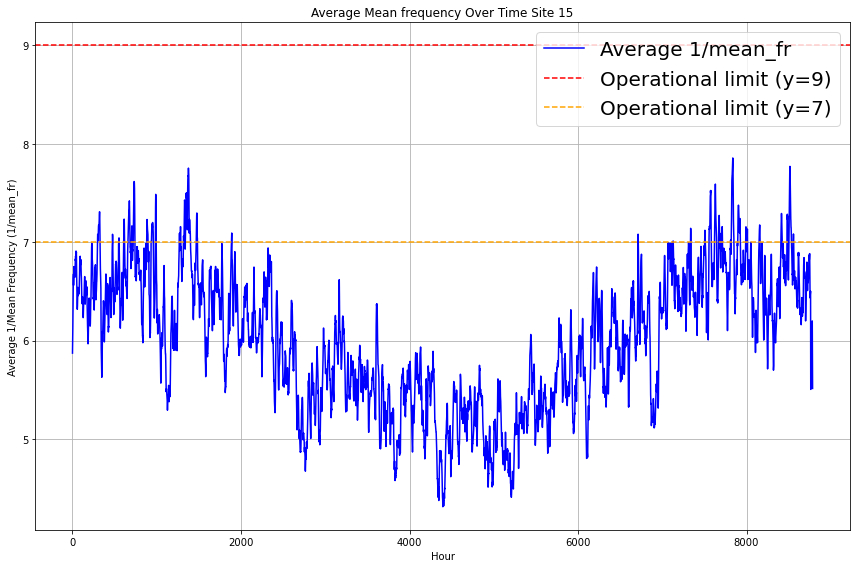
\includegraphics[width=\textwidth]{graphs/mean_fr_limit_site_15.png} 
        \caption{Mean Frequency}
        \label{fig:mean_fr_15}
    \end{subfigure}
    \vskip\baselineskip
    \begin{subfigure}[b]{0.47\textwidth}
        \centering
        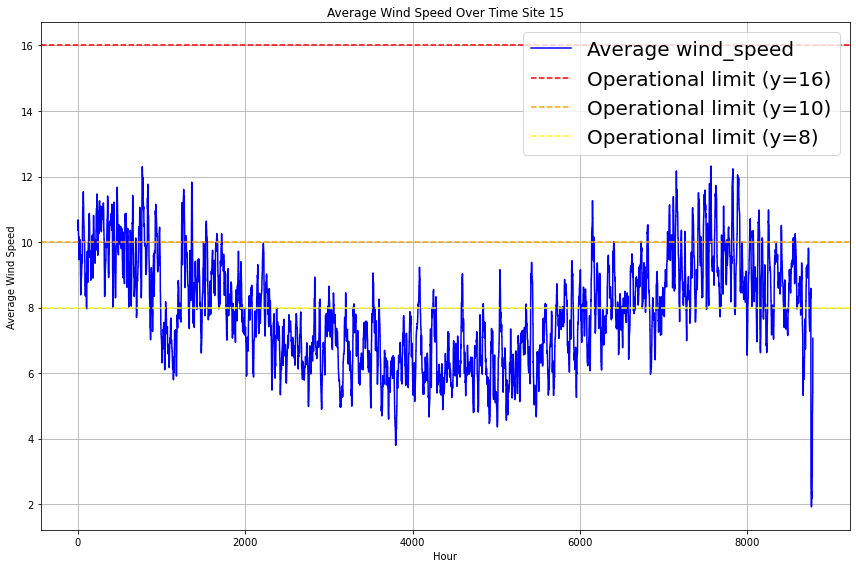
\includegraphics[width=\textwidth]{graphs/wind_speed_limit_site_15.png} 
        \caption{Wind Speed}
        \label{fig:wind_speed_15}
    \end{subfigure}
    \caption{Site 15 key parameters over time compared with operational limits}
    \label{fig:site15_limits}
\end{figure}

\newpage

\section{Mathematical Models}
\label{mathematical models}
This section will show the mathematical models specified for the inputted data and made for each model separately. To forecast the significant wave height ($s_{wht}$), the mean wave frequency ($mean_{fr}$), and the wind speed ($wind_{speed}$). 

\subsection{Mathematical model: Hybrid ARIMA–ANN Model}
\label{math:hybrid}
\noindent \textbf{ARIMA Component:}  
For each target variable, the ARIMA model is defined as:
\begin{equation}
    y(t) = \phi(B) \, y(t) + \theta(B) \, a_t,
    \label{eq:arima_generic}
\end{equation}
Where:
\begin{itemize}
    \item \(\phi(B)\) is the autoregressive polynomial,
    \item \(\theta(B)\) is the moving average polynomial,
    \item \(a_t\) denotes white noise,
    \item \(B\) is the backshift operator.
\end{itemize}

\noindent The residual error from the ARIMA model is computed as:
\begin{equation}
    e(t) = y(t) - \hat{y}_{ARIMA}(t),
    \label{eq:residual_error2}
\end{equation}
where \(\hat{y}_{ARIMA}(t)\) is the forecast produced by the ARIMA model.\\

\noindent \textbf{ANN Component:}  
The Artificial Neural Network (ANN) is used to model the nonlinear component of the time series. For a neuron \(j\) in layer \(l\), the activation is defined as:
\begin{equation}
    z^{(l)}_j = \sigma\left(\sum_{i=1}^{n_{l-1}} w_{ij}^{(l)} z_i^{(l-1)} + b_j^{(l)}\right),
    \label{eq:activation_function}
\end{equation}
Where:
\begin{itemize}
    \item \(w_{ij}^{(l)}\) and \(b_j^{(l)}\) are the weights and biases of layer \(l\),
    \item \(\sigma(\cdot)\) denotes an activation function (e.g., sigmoid or ReLU).
\end{itemize}

The output of the ANN is given by:
\begin{equation}
    y_{\text{ANN}}(t) = f(X),
    \label{eq:ann_output}
\end{equation}
with \(X\) representing a sliding window of past values from the same time series.\\

\noindent \textbf{Hybrid Forecast:}  
The final hybrid forecast is obtained by combining the ARIMA and ANN forecasts:
\begin{equation}
    y_{\text{hybrid}}(t) = \hat{y}_{ARIMA}(t) + y_{\text{ANN}}(t).
    \label{eq:hybrid_forecast2}
\end{equation}

\subsection{Mathematical model: Bayesian Neural Network with MC Dropout}
\label{math:BNN}

Let \( f(X, w) \) denote the output of a neural network for input \( X \) and weights \( w \). In our Bayesian Neural Network (BNN) framework, the weights are treated as random variables with an approximate posterior distribution \( q(w) \). Instead of performing full Bayesian inference, we use Monte Carlo Dropout to approximate this distribution during inference.\\

\noindent During a single forward pass with dropout active, the network function is computed as follows:
\begin{align}
    z^{(1)} &= \text{ReLU}(W^{(1)} X + b^{(1)}) \odot \xi, \label{eq:dropout_layer1}\\[1mm]
    z^{(2)} &= \text{ReLU}(W^{(2)} z^{(1)} + b^{(2)}), \label{eq:dropout_layer2}\\[1mm]
    \hat{y} &= W^{(3)} z^{(2)} + b^{(3)}, \label{eq:network_output}
\end{align}
Where:
\begin{itemize}
    \item \(W^{(l)}\) and \(b^{(l)}\) are the weight matrix and bias vector for layer \(l\),
    \item \(\text{ReLU}(\cdot)\) is the Rectified Linear Unit activation function,
    \item \(\xi\) is a dropout mask applied element-wise, with each element sampled from a Bernoulli distribution \(\text{Bernoulli}(1-p)\), where \(p\) is the dropout rate,
    \item The operator \(\odot\) denotes element-wise multiplication.
\end{itemize}

\noindent To approximate the predictive distribution, we perform \(N\) stochastic forward passes, each with independent dropout masks. The final prediction is obtained by averaging these Monte Carlo samples:
\begin{equation}
    \hat{y}_{\text{MC}} = \frac{1}{N} \sum_{i=1}^{N} f(X, w_i),
    \label{eq:mc_dropout_prediction}
\end{equation}
where each \(w_i\) represents a set of weights resulting from a different dropout mask.

\noindent This procedure approximates Bayesian inference by effectively sampling from the approximate posterior \(q(w)\) and provides both a mean prediction and a measure of uncertainty.

\subsection{Mathematical model: LSTM}
\label{math:LSTM}
The Long Short-Term Memory (LSTM) network is designed to capture both short-term fluctuations and long-term dependencies in time series data. An LSTM unit is defined by the following set of equations:
\begin{align}
    i_t &= \sigma\left(W_i x_t + U_i h_{t-1} + b_i\right), \label{eq:lstm_input}\\[1mm]
    f_t &= \sigma\left(W_f x_t + U_f h_{t-1} + b_f\right), \label{eq:lstm_forget}\\[1mm]
    o_t &= \sigma\left(W_o x_t + U_o h_{t-1} + b_o\right), \label{eq:lstm_output}\\[1mm]
    \tilde{C}_t &= \tanh\left(W_C x_t + U_C h_{t-1} + b_C\right), \label{eq:lstm_candidate}\\[1mm]
    C_t &= f_t \odot C_{t-1} + i_t \odot \tilde{C}_t, \label{eq:lstm_cell}\\[1mm]
    h_t &= o_t \odot \tanh\left(C_t\right), \label{eq:lstm_hidden}
\end{align}
where:
\begin{itemize}
    \item \(x_t\) is the input at time \(t\),
    \item \(h_t\) is the hidden state at time \(t\),
    \item \(C_t\) is the cell state at time \(t\),
    \item \(i_t\), \(f_t\), and \(o_t\) denote the input, forget, and output gates respectively,
    \item \(W_i, W_f, W_o, W_C\) are the weight matrices for the input,
    \item \(U_i, U_f, U_o, U_C\) are the recurrent weight matrices,
    \item \(b_i, b_f, b_o, b_C\) are the bias vectors,
    \item \(\sigma(\cdot)\) is the sigmoid activation function,
    \item \(\tanh(\cdot)\) denotes the hyperbolic tangent function,
    \item \(\odot\) represents element-wise multiplication.
\end{itemize}

For forecasting, a sequence-to-one architecture is employed:
\[
\hat{y}(t) = f_{\text{LSTM}}(x_{t-k}, \ldots, x_{t-1}),
\]
where \(\{x_{t-k}, \ldots, x_{t-1}\}\) is the input sequence of length \(k\) and \(\hat{y}(t)\) is the forecast at time \(t\).

\section{Flowchart}
\label{flowcharts}
To clarify the construction and operational framework of the forecasting models, flowcharts for each approach are presented. These diagrams serve as visual guides that outline the step-by-step development process, ensuring that each model is built systematically and functions as intended.

\begin{center}
\begin{tikzpicture}[node distance=0.5cm, auto,
    block/.style={draw, rectangle, rounded corners, fill=blue!20, align=center, minimum width=3cm, minimum height=1cm},
    arrow/.style={->, thick, >=stealth}]

    \node[block] (preprocess) {Data Preprocessing};
    \node[font=\bfseries, above=0.3cm of preprocess, align=center] (title) {Hybrid ARIMA–ANN Model Framework};
    \node[block, below left=of preprocess, xshift=-1.4cm] (arima) {ARIMA Model\\(Linear Forecast)};
    \node[block, below right=of preprocess, xshift=1.4cm] (ann) {ANN Model\\(Nonlinear Forecast)};
    \node[block, below=of preprocess, yshift=-1cm] (hybrid) {Hybrid Forecast\\\(\hat{y}_{ARIMA} + y_{ANN}\)};
    \node[block, below=of hybrid] (refit) {Model Refit \& Error Calculation};
    \node[block, below=of refit] (rolling) {Rolling Update\\ \& Forecasting Loop};
    \node[block, below=of rolling] (evaluation) {Evaluation};

    \draw[arrow] (preprocess) -- (arima);
    \draw[arrow] (preprocess) -- (ann);
    \draw[arrow] (arima) to node[above]{\shortstack{Residual error:\\ \(e(t)=y(t)-\hat{y}_{ARIMA}(t)\)}} (ann);
    \draw[arrow] (arima) -- (hybrid);
    \draw[arrow] (ann) -- (hybrid);
    \draw[arrow] (hybrid) -- (refit);
    \draw[arrow] (refit) -- (rolling);
    \draw[arrow] (rolling) -- (evaluation);
    
\end{tikzpicture}
\end{center}

\begin{center}
\begin{tikzpicture}[node distance=0.5cm, auto,
    block/.style={draw, rectangle, rounded corners, fill=blue!20, align=center, minimum width=3cm, minimum height=1cm},
    arrow/.style={->, thick, >=stealth}]

    \node[block] (preprocess_bnn) {Data Preprocessing};
    \node[block, below=of preprocess_bnn] (bnn) {BNN with MC Dropout\\(Stochastic Forward Passes)};
    \node[block, below=of bnn] (aggregation) {Aggregation of MC Samples\\(Final Forecast)};
    \node[block, below=of aggregation] (refit_bnn) {Model Refit \& Error Calculation};
    \node[block, below=of refit_bnn] (rolling_bnn) {Rolling Update \& Forecast Loop};
    \node[block, below=of rolling_bnn] (evaluation_bnn) {Evaluation};

    \node[above=0.3cm of preprocess_bnn, font=\bfseries] {BNN with MC Dropout Model};
    
    \begin{scope}[xshift=8cm]
        \node[block] (preprocess_lstm) {Data Preprocessing};
        \node[block, below=of preprocess_lstm] (lstm_train) {LSTM Training\\(Sequence-to-One)};
        \node[block, below=of lstm_train] (forecast_lstm) {LSTM Forecasting};
        \node[block, below=of forecast_lstm] (refit_lstm) {Model Refit \& Error Calculation};
        \node[block, below=of refit_lstm] (rolling_lstm) {Rolling Update \& Forecast Loop};
        \node[block, below=of rolling_lstm] (evaluation_lstm) {Evaluation};

        \node[above=0.3cm of preprocess_lstm, font=\bfseries] {LSTM Model};
    \end{scope}

    \draw[arrow] (preprocess_bnn) -- (bnn);
    \draw[arrow] (bnn) -- (aggregation);
    \draw[arrow] (aggregation) -- (refit_bnn);
    \draw[arrow] (refit_bnn) -- (rolling_bnn);
    \draw[arrow] (rolling_bnn) -- (evaluation_bnn);
    
    \draw[arrow] (preprocess_lstm) -- (lstm_train);
    \draw[arrow] (lstm_train) -- (forecast_lstm);
    \draw[arrow] (forecast_lstm) -- (refit_lstm);
    \draw[arrow] (refit_lstm) -- (rolling_lstm);
    \draw[arrow] (rolling_lstm) -- (evaluation_lstm);
    
\end{tikzpicture}
\end{center}

\newpage

\section{Model Development}
\label{model development}
This section describes how each model was built and trained, including the preprocessing, the hyperparameter choosing and the rolling refit strategies. 

\subsection{Data Preprocessing}
Before training the forecasting models and constructing the different scripts, it is essential to preprocess the inputted data. This needs to be done to ensure the learning algorithms of the models receive consistent and meaningful data. Five different steps are taken before the data can be used. Beginning with the handling of missing values, by implementing linear interpolation, these values can be estimated. When a value is not available, past values are used to bridge the gaps in the inputted data. Secondly, leap days are removed from the data, while this would give different sizes of inputted data, which will be mishandled by the models.\\

\noindent Each parameter is then scaled to normalise the inputted data. This is done to make the gradient-based optimizers in the scripts converge faster. The normalization parameters are then saved and will be used for the testing of the refitted data. A second reason to perform this normalization is to ensure that each variable exerts a balanced influence on the model.
The data is split into two, the years 2001-2008 will be used as training years for the models. The data for 2009-2010 will be used as the testing years. This clear split is done to ensure there is no accidental data leakage in the construction of the forecasts.\\

\noindent Finally, a refit interval of five days is used to be able to make a rolling forecast without exceeding the computational time. After each five days, the new observations of the actual data are added to the rolling windows. These rolling windows are then used to update the whole model, so instead of using all available data to reconstruct a new model, the old model is updated with this new data. 

\subsection{Hybrid ARIMA-ANN Model Development}
To develop the Hybrid model, the flowchart from Chapter \ref{flowcharts} and the mathematical model from Chapter \ref{math:hybrid} are used. Two site-by-site models need to be created, one for the linear components of the data and one for the non-linear components. This is all done to eventually forecast the significant wave height, $s_{wht}$, the mean wave frequency, $mean_{fr}$, and the wind speed $wind_{speed}$.\\ 

\noindent First, the ARIMA model, from Formula \ref{eq:arima_generic}, to find a good configuration between the autoregressive, diverging and moving average part, an iterative process is performed. During the process, it is found that [2 0 3] would give a minimal mean squared error concerning the actual data. The ARIMA is then fitted over the historical data and will produce a \(\hat{y}_{ARIMA}(t)\). This is used to then calculate the residuals, Formula \ref{eq:residual_error2}, which will capture the parts ARIMA did not forecast.\\

\noindent This residual, \(e(t)\), will be the input for the non-linear, ANN, component of the model. The different number of hidden layers inside the ANN is found through an iterative process, that is why \(s_{wht}\) will have 5 hidden neurons, but \(mean_{fr}\) and \(wind_{speed}\) will have 15 hidden neurons. A training function is the Levenberg-Marquardt algorithm, which has a maximum number of epochs, the upper limit on the number of training iterations, and an error goal. The algorithm minimizes the mean squared error by iteratively adjusting the network weights and biases, this is done until the error goal is reached or the maximum number of epochs is used (\cite{hagan1994training}). Then it is used to predict \(y_{ANN}(t)\), when combined with  \(\hat{y}_{ARIMA}(t)\) the final hybrid forecast is obtained with Formula \ref{eq:hybrid_forecast2}.

\subsection{Bayesian Neural Network with MC Dropout Model Development}
The BNN with MC dropout network was constructed based on the mathematical model in Chapter \ref{math:BNN}. Instead of separating linear and non-linear, the BNN with MC dropout will incorporate the uncertainty directly on the predictions.\\

\noindent The model designed construct a feed-forward neural network consisting of multiple hidden layers. Dropout layers are inserted between these hidden layers and will stay active during training. With the usage of MC dropout, the network is forced to randomly deactivate some neurons during each forward pass. This stochastic behaviour approximates sampling from an underlying posterior distribution over the network weights. 
During training, the network has the goal to minimize the mean squared error combined with the dropout. The reason this dropout is necessary is to prevent over-fitting. The configuration of the model, so the hidden layer structure, the maximum epochs, the dropout rate and the MC iterations, are found iteratively. Keeping a good balance between the models' accuracy and the computational time. The window size for \(s_{wht}\) and \(mean_{fr}\), so how much data is included during each forecast step, follows from the tides, which repeat every 149 hours (\cite{pugh1987tides}).\\

\noindent During the forecasting phase the model will perform multiple forward passes for each input. For input \(X\) this will lead to a set of outputs \(\{f(X,w_1),(f(X,w_2),...,(f(X,w_i)\}\). The final forecast is found by averaging all of these outputs using the Formula \ref{eq:mc_dropout_prediction}. Next to these forecasts, this will also give the variability among the predictions, which can be seen as the forecast uncertainty.

\subsection{LSTM Model Development}
Long Short-Term Memory model is designed to capture the short-term fluctuations and long-term dependencies of the inputted data. The LSTM model was constructed based on the flowchart, Chapter \ref{flowcharts} and the mathematical model Chapter \ref{math:LSTM}. As part of the data preprocessing for this model, input sequences are created with a sequence length of 48 hours. This can be related to the short-term trends in the met-ocean data. The reason to choose this two-day time-span follows from the weather patterns that can persist for multiple hours or even days. A sequence length of 48 hours allows the model to recognize storm development patterns, improving the ability to forecast extreme conditions more accurately. While longer sequences could capture extended dependencies, they must be balanced against computational cost. A 2-day window provides a reasonable trade-off between computational efficiency and forecasting accuracy. To ensure the long-term memory of the model is trained effectively, a 12-week rolling window is used. Both short-term fluctuations and long-term dependencies can be found in this weather window. In summary, for the short-term dependencies of the model, a 48-hour sequence is used. To capture the long-term dependencies, a 12-week rolling window is used, so the forecasts will be based on the most recent 12 weeks of data. \\

\noindent The LSTM architecture is designed to process the time series data efficiently. The hidden layers consist of 35 LSTM units, which will be constructed in the same manner as in Figure \ref{fig:LSTM}. Using fewer units may result in underfitting, where the model fails to capture important patterns in the data. While more units could be included, they do not significantly increase the accuracy, but they will increase the computational time. A fully connected layer is added in the model, this will ensure the dependencies in the past data are used to make a well-constructed final forecast. Finally, a regression layer is added, which minimizes the mean squared error (MSE) during training, reducing the overall difference between actual and predicted values. These layers contribute to a more accurate forecast model during the training phase.

\section{Evaluation Metrics}
\label{evaluation metrics method}
Each model makes a rolling forecast for each parameter separately, to compare these models to each other, evaluation metrics are used. The models are trained over the first 8 years of the available data, so from 2001 till 2008, this training is done based on minimizing the Mean Squared Error (MSE) in Formula \ref{eq:MSE2}. Although this is also used during the training, the metric itself is still useful to examine the accuracy of the models.

\begin{equation}
\label{eq:MSE2}
\text{MSE} = \frac{1}{N} \sum_{i=1}^{N} \left(y_i - \hat{y}_i\right)^2
\end{equation}

\noindent The Mean Absolute Error (MAE), Formula \ref{eq:MAE}, is used to reflect on the average magnitude of the forecast error. By using this metric, all deviations in the outcome will be treated equally. 

\begin{equation}
\label{eq:MAE}
\text{MAE} = \frac{1}{N} \sum_{i=1}^{N} \left|y_i - \hat{y}_i\right|
\end{equation}

\noindent Next to the MSE metric a Root Mean Squared Error (RMSE), Formula \ref{eq:RMSE}, like MSE, it will give a greater weight to larger errors. The reason to still use this follows from the fact that RMSE will penalize large errors more severely and so make it easier visible (\cite{hyndman2018forecasting}). 

\begin{equation}
\label{eq:RMSE}
\text{RMSE} = \sqrt{\frac{1}{N} \sum_{i=1}^{N} \left(y_i - \hat{y}_i\right)^2}
\end{equation}

\noindent Finally, to evaluate how accurate the forecast is to a naive baseline, a coefficient of determination ($R^2$), Formula \ref{eq:r^2}, is calculated. For this metric a value close to $1$ indicates the model captures a large part of the variance in the data. Negative values imply the model would be performing then the naive baseline (\cite{montgomery2012introduction}).

\begin{equation}
\label{eq:r^2}
R^2 = 1 - \frac{\sum_{i=1}^{N} \left(y_i - \hat{y}_i\right)^2}{\sum_{i=1}^{N} \left(y_i - \bar{y}\right)^2}
\end{equation}

%\section{Model Validation}
%\subsection{Validation Techniques}
%Description of various validation methods (e.g., cross-validation, holdout validation, time-series split) used for assessing model performance.

%\subsection{Training and Test Datasets}
%Explanation of how training and test datasets are selected and prepared.

%\subsection{Performance Metrics for Validation}
%Discussion of specific metrics used for validation (e.g., RMSE, MAE, R²) and their relevance in evaluating forecast accuracy.
